%\documentclass[a4paper]{article}
\documentclass[a4paper,fleqn,12pt]{JMThesis}
%%% These are PDF packages needed to include PDF pictures
\usepackage[pdftex]{graphicx}
\DeclareGraphicsExtensions{.pdf}


\usepackage[OT2]{fontenc}
\newcommand{\latin}{\fontencoding{T1}\selectfont}
\usepackage{minted}
\usepackage[toc,page]{appendix}
\usepackage{wrapfig}
\usepackage[serbian]{babel}

\usepackage{tabu}
\usepackage{longtable}
\renewcommand{\baselinestretch}{1}
\usepackage{amsfonts}
\usepackage{amssymb}
\usepackage{amsthm}
\usepackage{amsmath}
%\usepackage{gclc}
\usepackage{newlfont}
\usepackage{graphicx}
\usepackage{xcolor}
\usepackage{verbatim,enumerate}
\usepackage{wasysym}
\usepackage{mdwlist}
\usepackage{multicol}
%\input amssym.def
%\input amssym
\usepackage{fancyhdr}
\usepackage{tocloft}
\usepackage{listings}

% Pie chart drawing library 
\usepackage{pgf-pie}  
 

\definecolor{codegreen}{rgb}{0,0.6,0}
\definecolor{codegray}{rgb}{0.5,0.5,0.5}
\definecolor{codepurple}{rgb}{0.58,0,0.82}
\definecolor{backcolour}{rgb}{0.95,0.95,0.92}

% \lstdefinestyle{mystyle}{
%     backgroundcolor=\color{backcolour},   
%     commentstyle=\color{codegreen},
%     keywordstyle=\color{magenta},
%     numberstyle=\tiny\color{codegray},
%     stringstyle=\color{codepurple},
%     basicstyle=\ttfamily\footnotesize,
%     breakatwhitespace=false,         
%     breaklines=true,                 
%     captionpos=b,                    
%     keepspaces=true,                 
%     numbers=left,                    
%     numbersep=5pt,                  
%     showspaces=false,                
%     showstringspaces=false,
%     showtabs=false,                  
%     tabsize=2
% }

% \lstset{style=mystyle}

\lstset{ %
  language=bash,                  % the language of the code
  basicstyle=\footnotesize,       % the size of the fonts that are used for the code
  numbers=left,                   % where to put the line-numbers
  numberstyle=\tiny\color{gray},  % the style that is used for the line-numbers
  stepnumber=1,                   % the step between two line-numbers. If it's 1, each line
                                  % will be numbered
  numbersep=5pt,                  % how far the line-numbers are from the code
  backgroundcolor=\color{white},  % choose the background color. You must add \usepackage{color}
  showspaces=false,               % show spaces adding particular underscores
  showstringspaces=false,         % underline spaces within strings
  showtabs=false,                 % show tabs within strings adding particular underscores
  frame=single,                   % adds a frame around the code
  rulecolor=\color{black},        % if not set, the frame-color may be changed on line-breaks within not-black text (e.g. commens (green here))
  tabsize=4,                      % sets default tabsize to 2 spaces
  captionpos=b,                   % sets the caption-position to bottom
  breaklines=true,                % sets automatic line breaking
  breakatwhitespace=false,        % sets if automatic breaks should only happen at whitespace
  title=\lstname,                 % show the filename of files included with \lstinputlisting;
                                  % also try caption instead of title
  keywordstyle=\color{blue},          % keyword style
  commentstyle=\color{green},       % comment style
  stringstyle=\color{red},         % string literal style
  escapeinside={\%*}{*)},            % if you want to add a comment within your code
  morekeywords={git,*,...}               % if you want to add more keywords to the set
}

\usepackage[font=small,labelfont=bf]{caption}
%\captionsetup{figurewithin=section,tablewithin=section}

% \newcommand{\Z}{\symbol{'21}}
% \newcommand{\z}{\symbol{'31}}
% \newcommand{\ch}{\symbol{'161}}
% \newcommand{\Ch}{\symbol{'121}}
% \newcommand{\sh}{\symbol{'170}}
% \newcommand{\Sh}{\symbol{'130}}
% \newcommand{\tj}{\symbol{'17}}
% \newcommand{\Tj}{\symbol{'7}}
% \newcommand{\dz}{\symbol{'12}}


\newcommand\DS{\displaystyle}
\newcommand\TS{\textstyle}
\newcommand{\konj}[1]{\overline {\rule {0pt}{7pt}{#1}}\,}
\oddsidemargin 1cm

\evensidemargin 0cm

\textwidth 15cm
% \textheight 21cm \topmargin 0.2cm

\definecolor{Light}{gray}{.80}
\definecolor{Dark}{gray}{.20}

\pagestyle{headings}



%\font\cyr=wncyr10 %scaled 1095,1200,1440 - povecavanje %
%slova d2 c1 ch sh zh dj lj nj
%wncyr10, wncyi10(italik),dncui10, wncyss10,wncysc10, %wncyb1
%\cyr  posle u tekstu
% 
\font \cyr=wncyr10 at 11pt
% 
% 
% \font \cyb=wncyb10 at 11pt
% 
% \font \cybbb=wncyb10 scaled 1300
% 
% \font \cybbbb=wncyb10 scaled 1400
% 
% \font \cybb=wncyb10 scaled 1800
% 
% \font \cyi=wncyi10 at 11pt
% 
% \font \cysc=wncysc10 at 11pt
% 
% \font \cyss=wncyss10 at 11pt
% 
\font \matematicka=wncsc10 scaled 1600
% 
 \font \maturski=wncyb10 scaled 2500
% 
 \font \naslov=wncyb10 scaled 1900
% 
 \font \imen=wncyr10 scaled 1600


\theoremstyle{plain}

\theoremstyle{definition}

 \newtheorem{pr}{Primer}
 \newtheorem{te}{Teorema}[chapter]
 \newtheorem{teo}{Teorema}[section]
 \newtheorem{lem}{Lema}[chapter]
 \newtheorem{lema}{Lema}[section]
 \newtheorem{po}{Posledica}
 \newtheorem{de}{Definicija}[section]
 \newtheorem{za}{Zadatak}
 \newtheorem{reza}{Reshenje}
 \newtheorem{fm}{F}

\newcommand{\dok}{\noindent \textit{Dokaz:}}

\renewcommand\lstlistingname{Izvorni kod}


\newcommand{\zbn}{\sum_n}
\newcommand{\zbng}{\sum_{n=0}^\infty}
\newcommand{\zbk}{\sum_k}
\newcommand{\zbkg}{\sum_{k=0}^\infty}
\newcommand{\zbi}{\sum_i}
\newcommand{\zbig}{\sum_{i=0}^\infty}
\newcommand{\zbj}{\sum_j}
\newcommand{\zbjg}{\sum_{j=0}^\infty}
\newcommand{\osr}{\,_{\,\leftrightarrow}^{osr}\,}
\newcommand{\esr}{\,_{\,\leftrightarrow}^{esr}\,}

\newcounter{cpp}
\lstnewenvironment{cpp}[2]{
    \renewcommand\lstlistingname{Izvorni kod}
    \setcounter{lstlisting}{\value{cpp}}
    \lstset{ ... }
} {\addtocounter{cpp}{1}}

\newcounter{bash}
\lstnewenvironment{bash}[2]{
    \renewcommand\lstlistingname{Komanda}
    \setcounter{lstlisting}{\value{bash}}
    \lstset{ ... }
} {\addtocounter{bash}{1}}

%\renewcommand{\refname}{\cybb Literatura}

%\newcommand{\clo}{\operatorname{\cl}\, }
\def\zn{,\kern-0.09em,}
\def\zng{'\kern-0.09em'}
\pagenumbering{roman}
%\mag=1200
\begin{document}

% \thispagestyle{empty}
% \textcolor{white}{proba}
% \clearpage

\thispagestyle{empty}

\begin{center}
{\matematicka Matematichka gimnazija}
\end{center}
\vspace*{50mm}

\begin{center}
{\maturski MATURSKI RAD}

\vspace*{8pt}
{\naslov - iz Rachunarstva i informatike -}
\end{center}

\vspace*{10pt}
\begin{center}
{\naslov Softver otvorenog koda i njegove primene}



\end{center}

\vspace*{70mm}
\setlength{\columnsep}{50pt}
\begin{multicols}{2}
 {\noindent \imen Uchenik:
\\Nikola Drakulic1  $\operatorname{IV}$c}


{ \noindent \hfill \imen Mentor:\\
\hfill \phantom{aa} Mijodrag Djurishic1 }
\end{multicols}

\vfill
\begin{center}
{\imen Beograd, jun 2021.}
\end{center}
\newpage
\clearpage

\thispagestyle{empty}
\textcolor{white}{proba}

\newpage


\renewcommand{\contentsname}{Sadrzhaj}
\thispagestyle{empty}

\pagenumbering{gobble}

\tableofcontents \clearpage

\thispagestyle{empty}
\textcolor{white}{proba}
\clearpage

%\pagestyle{fancy} %\lhead{\cyr Borsuk-Ulamova teorema i primene}
%\fancyhead[RE,RO]{\thepage}
\pagenumbering{arabic}
\renewcommand{\chaptername}{}
\setcounter{page}{1}
\chapter[Uvod]{Uvod}
Od nastanka rachunarskih nauka trazhe se nachini za efikasnu i jednostavnu saradnju izmedju programera. 
Lako je zakljuchiti da ukoliko bi svaki programer pisao sve od pochetka, pravljenje i najednostavnijih programa bi zahtevalo veliku kolichinu vremena. 
U ovom radu posvetic1emo se inicijativi otvorenog koda ({\latin Open Source Initiative - OSI }) koja je nastala 1998. 
{\latin OSI} su predvodili  {\latin Jon Hall, Larry Augustin, Eric S. Raymond, Bruce Perens}. 
Razmotric1emo istoriju, alate koji se koriste kao i kako se danas taj koncept primenjuje na sve vec1em broju projekata gde su neki od najznachajnijih {\latin Linux, Firefox, MySQL} i josh mnogi drugi. \par
Na primeru c1e se objasniti korish\-c1enje osnovnih alata, kontribucija projektu otvorenog koda i pravljene istog.




%%%%%%%%%%%%%%%%%%%%%%%%%%%%%%%%%%%%%%%%%%%%%%%%%%%%%%%%%%%%%%%%
%%%%%%%%%%%%%%%%%%%%%%%%%%%%%%%%%%%%%%%%%%%%%%%%%%%%%%%%%%%%%%%%
\chapter[Softver otvorenog koda]{Softver otvorenog koda}
\bigskip

%%%%%%%%%%%%%%%%%%%%%%%%%%%%%%%%%%%%%%%%%%%%%%%%%%%%%%%%%%%%%%%
%%%%%%%%%%%%%%%%%%%%%%%%%%%%%%%%%%%%%%%%%%%%%%%%%%%%%%%%%%%%%%%
%%%%%%%%%%%%%%%%%%%%%%%%%%%%%%%%%%%%%%%%%%%%%%%%%%%%%%%%%%%%%%%
%%%%%%%%%%%%%%%%%%%%%%%%%%%%%%%%%%%%%%%%%%%%%%%%%%%%%%%%%%%%%%%
Organizacaija \zn Inicijativa otvorenog koda" je definisala softver otvorenog koda kao bilo koji izvorni kod napravljen pod jednom od licenci iz liste dozvoljenih licenci. 
Neke od najpoznatijih licenci iz te liste su sledec1e:
\begin{itemize}
{\latin
    \item Apache License 2.0
    \item BSD 3-Clause "New" or "Revised" license
    \item BSD 2-Clause "\-Simplified" or "FreeBSD"  license
    \item GNU General Public License (GPL)
    \item MIT license
    \item Mozilla Public License 2.0
    \item Common Development and Distribution License
    \item Eclipse Public License version 2.0
    }
\end{itemize}
Iako licence medjusobno nisu iste sve lincece omoguc1avaju pristup izvornom kodu nekog programa kao i njegovu modifikaciju, dok je razlika na koji je nachin omoguc1ena dalja distribucija. 
%neke razlike u licencama
\section[Istorija]{Istorija}
\medskip

U aprilu 1991 godine, {\latin Linus Torvalds}, tadashnji student finskog univerziteta u Helsiniju, krec1e da radi na, u tom trenutku, malom projektu koji je trebao da bude kopija kernela, tadashenjeg {\latin Minix} operativnog sistema pod nazivom {\latin Linux}.
U avgustu iste godine objavljuje prvu verziju programa koja je podrzhavala {\latin Bash} koji je jezik za pisanje skripti i kompajler za programski jezik {\latin C} - {\latin gcc} iz {\latin GNU} projekta.
U njegovim opisima verzija je zabelezhio da c1e {\latin Linux} podrzhavati samo arhitekturu AT-386 kako je to bio rachunar na kome je radio.
Naveo je da {\latin Linux} nec1e biti nishta profesionalno kao shto je to {\latin GNU} projekat. \par
Dva meseca kasnije u verziji 0.02 {\latin Linux} je mogao da pokrene vec1inu programa iz projekta {\latin GNU}.
Kompletan kod za kernel bio je dostupan na univerzitet\-skom sajtu.\par

Baza korisnika {\latin linux}-a je mahom bila sastavljena od osoba koje su imale programerskog iskustva.
Korisnici su ubrzo pocheli da koriste i da prave svoje izmene na kernelu koje su slali nazad Linusu, koji je te izmene unosio u kernel.
Takav nachin razvijanja softvera bio je u protivljenu standardima i navikama vec1ine ljudi. \par
{\latin GNU} projekat, koji je za cilj imao da napravi kompletan operativni sistem, izdavao je sa svakom verzijom ceo izvorni kod, ali je metodika rada bila drugachija. 
Smatrano je da na programu treba da radi mali broj ljudi koji c1e pazhljivo dodavati svaku novu moguc1nost.
Verzije programa bi izlazile na svakih par meseci. \par

Nasuprot tome Torvalds je prihvatao kod od velikog broja ljudi i verzije su izlazile vishe puta nedeljno. 
Takav nachin rada doveo je do mnogo testera koda koji su znachajno brzhe nalazili kako probleme tako i reshenja tih problema u odnosu na stil pravljenja koji se do tada koristio.\par
Do ovih zakljuchaka je u svom eseju, pod nazivom \zn {\latin The Cathedral and the Bazaar}", doshao Erik Raimond. 
Rad je izazvao mnogo pazhnje i doveo da kompanija {\latin  Netscape Communications Corporation} izbaci svoju pretechu internet pretra-zhivacha kao besplatan softver. Iz njega su se kasnije razvili {\latin Firefox} - jedan od najvec1ih pretrazhivacha i {\latin Thunderbird} e-mail klijent za {\latin Linux}.

\section[Softver otvorenog koda danas]{Softver otvorenog koda danas}
\medskip

Zastupljenost aplikacija otvorenog koda je u porastu. Krajnji korisnici aplikacija idalje biraju aplikacije zatvorenog koda pre aplikacija otvorenog koda ali razvijachi softvera se u sve vec1oj meri odluchuju za {\latin linux} i alatke koje su otvorenog koda. \par
Na personalnim rachunarima {\latin linux} operativni sistem zuzima samo 2.18\% slika (\ref{fig:mspc}). 
Na serverima je zastupljnost {\latin linux} kernela 75.3\% dok je na super rachunarima upotpunosti zastupljen {\latin linux.}
\begin{figure}
    \centering
    \begin{tikzpicture}
    \pie{
    74.96/{\latin Windows},
16.02/{\latin OS X},
4.81/{\latin Unknown},
2.18/{\latin Linux},
2.02/{\latin Chrome OS}
}
    \end{tikzpicture}
    \caption{Trzhshni udeo operativnih sistema za personalne rachunare}
    \label{fig:mspc}
\end{figure}

Vec1ina mobilnih uredjaja za operativni sitem ima {\latin Android}(72,2\%) koji je nastao kao zasebna grana {\latin linux} kernela koju danas odrzhava {\latin Google}. 
U tabeli (\ref{table:poredjenje}) mozhemo da vidimo pregled popularnih programa u svakodnevoj upotrebi kao i alternative otvorenog koda.  
{\tabulinesep=3mm
\begin{longtabu}{ |  X[ 3 , c ] | X[ 2 , c ] |X[ 2 , c ] | } 
\hline
\textbf{Opis programa} & \textbf{Programi zatvorenog koda} & \textbf{Programi otvorenog koda}
 \hline
Paket programa za kancelariju &{\latin Microsoft Office} & {\latin OpenOffice}, {\latin LibreOffice} \\ 
  \hline
 Obrada slika &{\latin Adobe Photoshop} & {\latin GIMP} \\ 
 \hline
 Vektorske grafike &{\latin Adobe Ilustrator} & {\latin Inkscape} \\ 
 \hline
 Pravljenje video igara &{\latin Unity}, {\latin Unreal Engine} & {\latin Godot} \\
 \hline
 Inzhenjersko crtanje &{\latin AutoCAD} & {\latin FreeCAD} \\
 \hline
 Internet pretrazhivachi &{\latin Google Chrome} & {\latin Firefox} \\
 \hline
\caption{Pregled alternativa otvorenog koda}
\label{table:poredjenje}
\end{longtabu}
}



\chapter[Git]{Git}
\bigskip

\section{Sistemi za kontrolu verzije}

U pochetku se sva saradnja vrshila pomoc1u razmene mejlova i ruchnog umetanja koda drugih programera. 
Vremenom su se razvili sistemi koji pomazhu da se na sistematichan nachin razvija kod i saradjuje sa vishe programera. 
Takve sisteme nazivamo sistemi za kontrolu verzija ({\latin Version Control System}-SKV). 
Prvi program koji predhodi modernim SKV je IBM-ov {\latin IEBUPDTE} napravljen 1962 godine za arhitekturu {\latin OS/360}.
Ovaj program je automat\-ski nadogragdjivao postojec1i kod pomoc1u fajla koji je u sebi ima linije koje je potrebno izmeniti, slichno programu {\latin patch} na modernim {\latin linux} sistemima. 
1972 godine za istu platformu izashao je program {\latin Source Code Control System (SCCS)} koji se smatra prvim pravim sistemom za kontorlu verzija. 
{\latin Revision Control System (RCS)} zamenjuje {\latin SCCS}. 
Prednosti {\latin RCS}-a su shto je omoguc1avao kontrolu projekta i na mrezhi a ne samo na jednom rachunaru. \par 

Jedan od trenutno najpopularnijih SKV je Git. 
Napravljen je od strane Linus Torvalds-a, 2005 godine, kao odgovor na promene u nachinu rada {\latin BitKeeper}-a.
Koji je do tada korish\-c1en za odrzhavanje {\latin Linux} kernela.
U pochetku je to trebao da bude samo sistem niskog nivo koji je trebao da zadovoljava sledec1e stavke:
\begin{itemize}
    \item Grafovska struktura
    \item Ne linearni rad mnogo programera - moguc1nost da postoje razlichite grane u verzijama
    \item Da ne koristi novi zatvoreni protokol
    \item Efikasnost na velikim projektima
    \item Ochuvanje integriteta i nemoguc1nost da se korumpiraju fajlovi
    \item Pakovanje objekata
\end{itemize}

Kasnije su napravljene i komande viskog nivoa pomoc1u kojih je moguc1e da se git koristi efikasno bez potrebe za dodatnim programima

\section{Proces rada sa gitom}
Kako bi smo koristili git u projektu potrebno je da inicijalizujemo repozitorijum (za potrebe demostracije ime projekta c1e biti {\latin project}. Linije koje pochinju sa {\latin >} su linije koje {\latin bash} izvrshava a linije bez {\latin >} su povratne informacije komande)

{\latin
\begin{center}
\begin{lstlisting}[caption={\latin git init}]
> git init
Initialized empty Git repository in ~/project/.git/
\end{lstlisting}
\end{center}
}
{\latin git init} pravi u trenutnom direktorijumu folder {\latin ./.git} u kome se chuvaju sve potrebne informacije za dalji rad repozitorijuma. 
Dodajmo dva fajla {\latin test.cpp} i {\latin test.h} sa sledecim sadrzajem
{\latin
\begin{center}
    \begin{lstlisting}[language=C++,caption={\latin test.h}]
void triangle(int);
    \end{lstlisting}
\end{center}
}

{\latin
\begin{center}
    \begin{lstlisting}[language=C++,caption={\latin test.cpp}]
#include<iostream>
#include "test.h"

using namespace std;

void triangle(int n)
{
    for(int i = 1; i <= n;i++)
    {
        for(int j = 1;j <= i;j++)
            cout << "*";
        cout << endl;
    }
}

int main()
{
    triangle(4);
}
    \end{lstlisting}
\end{center}
}


Komanda {\latin git status} vrac1a:
\begin{itemize}
    \item Trenutnu granu na kojoj se nalazimo
    \item Fajlove koji su dodati u komit
    \item Promenjene fajlove koji mogu da se dodaju u komit
    \item Fajlove koji su promenjeni i koje idalje ne pratimo 
\end{itemize}

{\latin
\begin{center}
\begin{lstlisting}[caption={\latin git status}]
> git status
On branch master

No commits yet

Untracked files:
  (use "git add <file>..." to include in what will be committed)
        a.out
        test.cpp
        test.h

nothing added to commit but untracked files present (use "git add" to track)
\end{lstlisting}
\end{center}
}
Primetimo da git izlistava i fajl {\latin a.out} koji je kompajlovani program. 
Kompajlovani fajlovi se menjaju i ne znachi nam da chuvamo njihove verzije.
Git omoguc1ava da ignorishemo fajlove koji nemaju potrebe da se chuvaju pravljenjem fajla {\latin .gitignore} i zapisivanjem imena fajlove i foldera koje git treba da ignorishe.

{\latin
\begin{center}
\begin{lstlisting}[caption={\latin .gitignore}]
*.out
\end{lstlisting}
\end{center}
}
Ovim c1e git zanemarivati sve fajlove koji se zavrshavaju sa ekstenzijom {\latin out}.


{\latin
\begin{center}
\begin{lstlisting}[caption={\latin git status}]
> git status
On branch master

No commits yet

Changes to be committed:
  (use "git rm --cached <file>..." to unstage)
        new file:   .gitignore
        new file:   test.cpp
        new file:   test.h
\end{lstlisting}
\end{center}
}

Kako bi smo sachuvali izmene potrebno je da dodamo fajlove pomoc1u ko-mande {\latin git add} i lista fajlova koje zhelimo da sachuvamo. 
Sada kada izvrshimo komandu {\latin git status} mozhemo da vidimo da imamo tri fajla koja su spremna za komit.
Za pravljenje komita koristi se {\latin git commit} sa parametrom {\latin -m} posle kojeg ide opis komita.

{\latin
\begin{center}
\begin{lstlisting}[caption={\latin git commit}]
> git commit -m "prvi komit"
[master (root-commit) f15df41] prvi komit
 3 files changed, 21 insertions(+)
 create mode 100644 .gitignore
 create mode 100644 test.cpp
 create mode 100644 test.h
\end{lstlisting}
\end{center}
}
Iz rezultata komande mozhemo da prochitamo sledec1e. 
Na grani {\latin master} napravili smo prvi komit sa nazivom prvi komit. 
Broj {\latin f15df41} je skrac1eni id komita i pomoc1u njega mozhemo da se vratimo na odredjeni komit. 
Skrac1eni id je nastao od prvih 7 cifara celog id-a.
Ceo id se generishe kao {\latin SHA-1} hesh komita.  
Git chuva sve komitove kao orjentisani aciklichni graf.
Podrazumevno ime glavna grane grafa je {\latin master}. 
Svaki komit pored promena u fajlovima chuva autora i vreme kada je napravljen komit. 
Komandom {\latin git log} mozhemo da vidimo sve prethodne komitove. {\latin HEAD} je pokazivach na zadnji komit na trenutnoj grani.
{\latin
\begin{center}
\begin{lstlisting}[caption={\latin git log}]
> git log
commit f15df41fb0e4621e26ed3757f10c576c3a9f3482 (HEAD -> master)
Author: Drakula44 <ninadrakulic04@gmail.com>
Date:   Sat May 22 15:34:51 2021 +0200

    prvi komit
\end{lstlisting}
\end{center}
}
Ukoliko vishe programera radi na jednom projektu praksa je da svaki programer radi na posebnoj grani kako bi se izbegli konflikti.\par
Kreiranje nove grane se izvrshava komandom {\latin git checkout -b} pa ime grane. Napravimo granu kvadrat i dodajmo moguc1nost da kod ispisuje i kvadrate zadate velichine. Komandom {\latin git diff} mozhemo da vidimo promene koje smo napravili u odnosu na proshli komit.

{\latin
\begin{center}
\begin{lstlisting}[caption={\latin git diff}]
> git diff
diff --git a/test.cpp b/test.cpp
index 658b2d2..44b083c 100644
--- a/test.cpp
+++ b/test.cpp
@@ -13,6 +13,16 @@ void triangle(int n)
     }
 }

+void square(int n)
+{
+    for(int i = 1; i <= n;i++)
+    {
+        for(int j = 1;j <= n;j++)
+            cout << "*";
+        cout << endl;
+    }
+}
+
 int main()
 {
     triangle(4);
diff --git a/test.h b/test.h
index dbc8590..ab917eb 100644
--- a/test.h
+++ b/test.h
@@ -1 +1,2 @@
-void triangle(int);
\ No newline at end of file
+void triangle(int);
+void square(int);
\ No newline at end of file
\end{lstlisting}
\end{center}
}

Linije koda koje ispired sebe imaju {\latin +} su dodate dok su one sa {\latin -} izbrisane.
Neka je ovo novi komit na grani kvadrat. 
Paralelno je na grani {\latin master} dodat komit koji omoguc1ava unoshenje velichine trougla iz komandne linije. 
Spajanje grane {\latin kvadrat} sa granom {\latin master} postizhe se komandom {\latin git merge} pa ime grane koju spajamo sa trenutnom. 
Tako se zapochinje proces spajanja.
Git c1e pokushati da automat\-ski spoji sve promene gde se linije koje su promenjene ne poklapaju.
Ukoliko to nije moguc1e potrebno je ruchno izabrati promene koje se prihvataju. 
Git c1e u fajlovima gde postoje konflikti ubaciti sve promene pa mi mozhemo da odluchimo koje c1emo promene da prihvatimo.

{\latin
\begin{lstlisting}[language=C++,caption=izgled {\latin test.cpp} fajla koji treba ruchno da se spoji]
#include<iostream>
#include <cstdlib>
#include "test.h"

using namespace std;

void triangle(int n)
{
    for(int i = 1; i <= n;i++)
    {
        for(int j = 1;j <= i;j++)
            cout << "*";
        cout << endl;
    }
}

<<<<<<< HEAD
int main(int argc, char *argv[])
=======
void square(int n)
{
    for(int i = 1; i <= n;i++)
    {
        for(int j = 1;j <= n;j++)
            cout << "*";
        cout << endl;
    }
}

int main()
>>>>>>> kvadrat
{
    int n = atoi(argv[1]);
    triangle(n);
}
\end{lstlisting}
}

Kada izvrshimo spajanje potrebno je da napravimo komit koji c1e predstavljati zavrshetak spajanja. Na slici (\ref{fig:komitovi}) je prikazan graf komitova koji su napravljeni za potrebe ove demonstracije.

\begin{figure}[H]
    \centering
    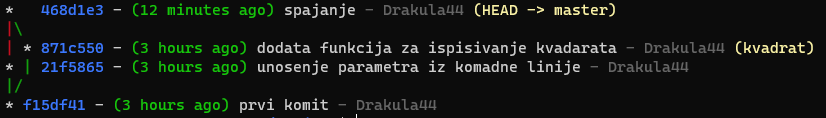
\includegraphics[scale=0.7]{komitovi.png}
    \caption{Prikaz komitova}
    \label{fig:komitovi}
\end{figure}

\section{Hosting projekta}

Kako bi vishe ljudi moglo da radi na istom projektu potrebno je da repozitorijum bude na serveru koji c1e predstavljati mesto odakle mozhe da se preuzme a kasnije i postave nadogradnje projekta. 
Na internetu postoji mnoshtvo sajtova koji pruzhaju takve usluge. Jedan od najpopularnijih je {\latin GitHub}.
Kako bi smo postavili svoj projekat na {\latin GitHub} prvo je potrebno da napravimo projekat na njihovom sajtu.

\begin{figure}[H]
    \centering
    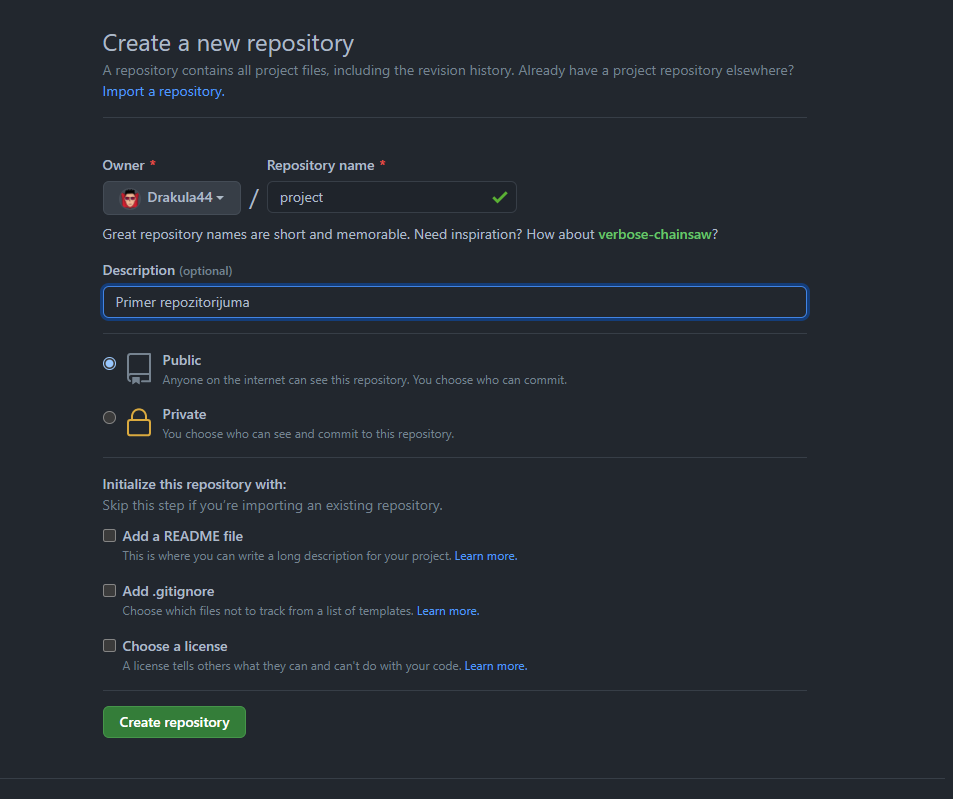
\includegraphics[scale=0.4]{pravljenje repa.png}
    \caption{Pravljenje repozitorijuma u {\latin Github}-u}
    \label{fig:pravljenje-rep}
\end{figure}

Nakon napravljenong rezpozitorijuma na {\latin Gihub-u} potrebno je da podesimo udaljeni repozitorijum u nashem lokalnom. Komandom

{\latin
\begin{center}
\begin{lstlisting}[caption={\latin git remote add}]
>git remote add origin https://github.com/Drakula44/project.git
\end{lstlisting}
\end{center}
}

dodajemo udaljeni repozitorijum. Sa njim mozhemo da komuniciramo na tri osnovna nachina:
\begin{itemize}
    \item {\latin git fetch} - pomoc1u koje se proverava koje promene postoje na udaljenom repozitorijumu
    \item {\latin git pull} - preuzimamo promene nastale na udaljenom repozitorijumu
    \item {\latin git push} - shaljemo nashe nadogradnje na udaljeni repozitorijum
\end{itemize}

Kako na {\latin GitHubu-}u trenutno ne postoji ni jedna grana potrebno je da izvrshimo komandu:
{\latin
\begin{center}
\begin{lstlisting}[caption={\latin git push}]
git push origin --all
\end{lstlisting}
\end{center}
}

{\latin Origin} je naziv koji smo dali nashem udaljenom repozitorijumu dok parametar {\latin --all} govori da se poshalju promene sa svih grana.


\chapter[Primer kontribucije softveru otvorenog koda]{Primer kontribucije softveru otvorenog koda}

U ovom delu pogledac1emo proces ispravljanja greshke u kodu koja je uradjena za {\latin Microsoft}-ovu aplikaciju otvorenog koda {\latin PowerToys}.
\section{O {\latin PowerToys}-u}\par
{\latin PowerToys} je aplikacija sachinjena od par pod aplikacija sa namerom da donese neke dodatne moguc1nosti naprednim korisnicima {\latin Windows 10} operativnog sistema. Lista pod aplikacija:
\begin{itemize}
    \item {\latin Color Picker} - alatka za ochitavanje trenutne boje nekog piksela sa ekrana
    \item {\latin FancyZones} - napredna organizacija otvorenih prozora i njihovo ponashanje
    \item {\latin File Explorer Add-ons} - dodatne opcije za pretrazhivach datoteka {\latin File\\ Explorer}.
    \item {\latin Image Resizer} - alatka u kontekst meniju za generisanje slika drugachijih rezolucija
    \item {\latin Keyboard Manager}	- omoguc1ava zamenu tastera i prechica.
    \item {\latin PowerRename} - alatka za masovno preimenovanje fajova
    \item {\latin PowerToys Run} - multi funkcionalni pretrazhivachki alat.
    \item {\latin Shortcut Guide} - pregled svih prechica koje su ugradjene u {\latin Windows 10} operativnom sistemu.
\end{itemize}

\section{Unutrashnje funkcionisanje {\latin PowerToys}-a}
Kako bi doprineli nekom kodu potreno je da prvo razumemo nachin funkcionisanja do tadashnjeg koda. 
{\latin PowerToys} ima modularni dizajn. 
Svaki modul ima zaseban projekat i deo u korisnichkom interfejsu koji je pisan u {\latin C\#} programsom jeziku. 
Zasebni delovi modula se pokrec1u kao posebni procesi i komuniciraju sa korisnichkim interfejsom pomoc1u {\latin JSON} formata. 
Pogledajmo {\latin File Explorer Add-ons} prikaz korisnichkog  interfejsa slika (\ref{fig:set-fe}). Primetimo da se modul sastoji iz dve funkcije jedna dodaje dodatne tipove fajlove koje je moguc1e prikazati u panelu za pregled u {\latin File Explorer}-u, dok druga generishe slichice za dodatne tipove podataka.
Savostalan deo modula je napsian u {\latin C\#} programskom jer je pomoc1u njega moguc1e napraviti dodatne ekstenzije za {\latin File Explorer}.
\begin{figure}[H]
    \centering
    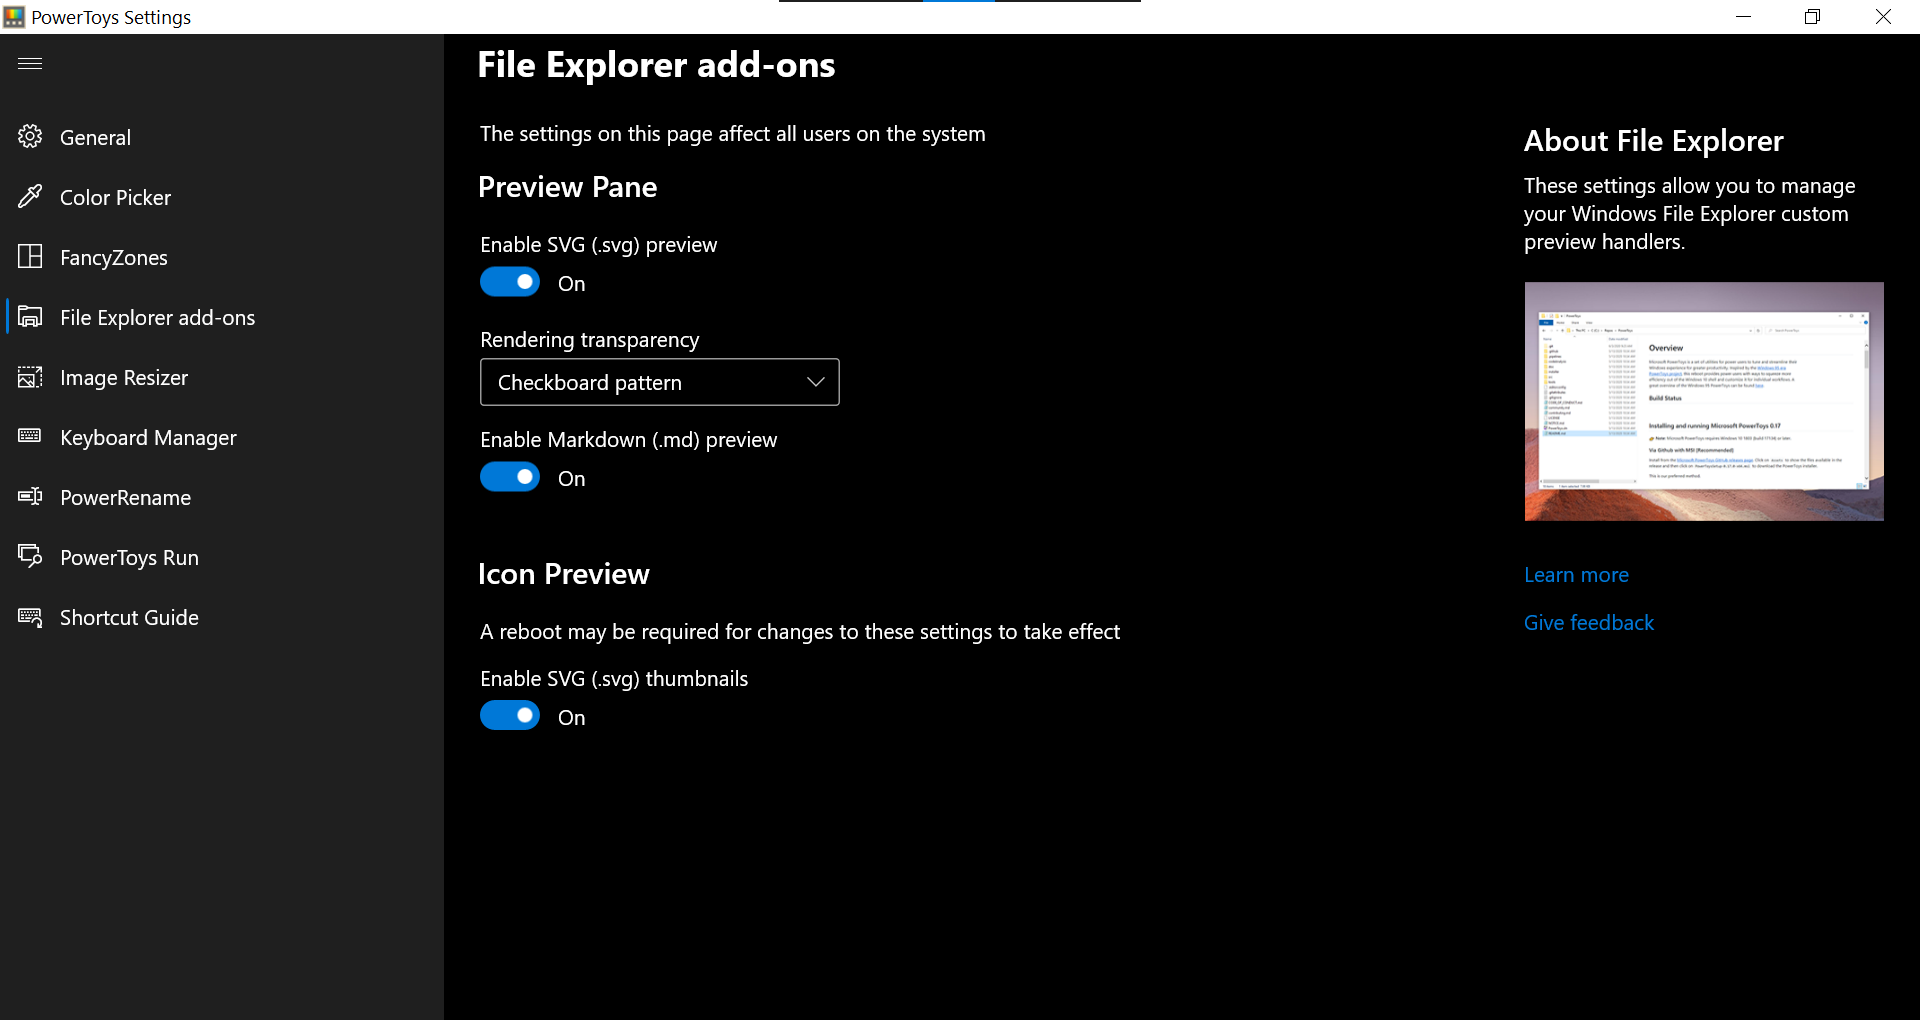
\includegraphics[scale=0.3]{settings-filexplorer.png}
    \caption{Korisnichki interfejs {\latin PowerToys}-a}
    \label{fig:set-fe}
\end{figure}
Pregledanje {\latin .svg} i {\latin .md} fajlova je panelu za pregled je realizovano pomoc1u biblioteke {\latin System.Windows.Forms.WebBrowserBase} za renderovanje internet stranica.

\section{Prijavljivanje problema}
U sklopu {\latin Github} repozitorijuma postoji sekcija {\latin Issues} u kojoj prijavljeni korisnici stranice mogu da prijave probleme vezane za aplikaciju.
\par Korisnik {\latin PrzemyslawTusinski} je primetio da prilikom renderovanja {\latin .svg} fajla prikaz se pojavljivao necentriran i neskaliran slika (\ref{fig:problem}). 
\begin{figure}[H]
    \centering
    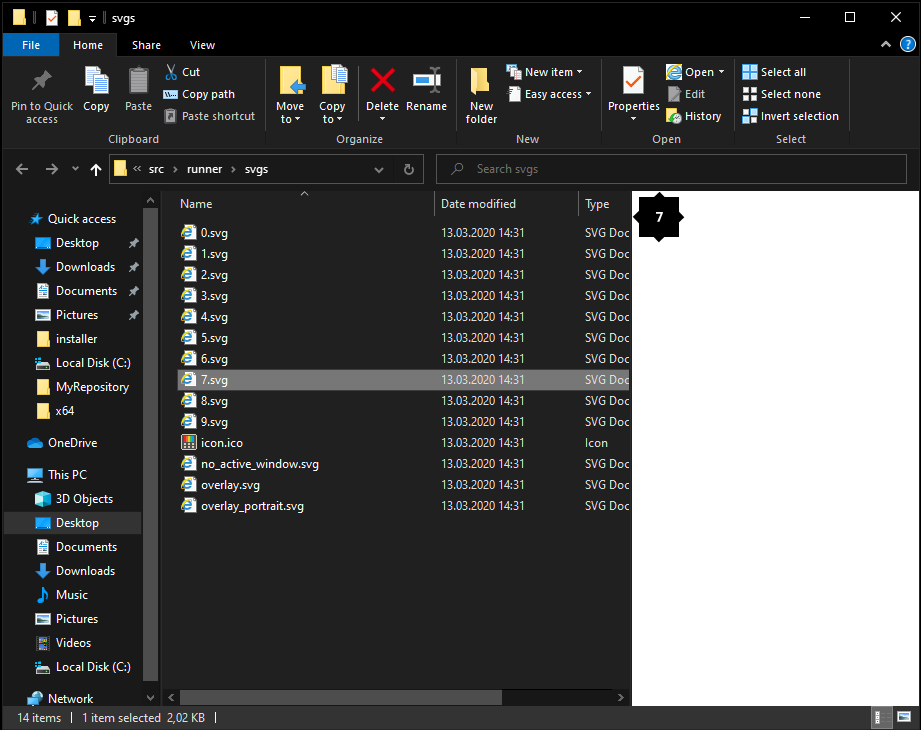
\includegraphics[scale=0.5]{issueproblem.png}
    \caption{Prikaz prijavljenog problema}
    \label{fig:problem}
\end{figure}
To nije oponashalo nachin na koji je prikazivanje slika radilo u {\latin File Explorer}-u i obelezheno je kao gresha za koji je trebala pomoc1. Ja sam se javio da imam zelju da pomognem oko ove greshke, slika (\ref{fig:prijava}).
\begin{figure}[H]
    \centering
    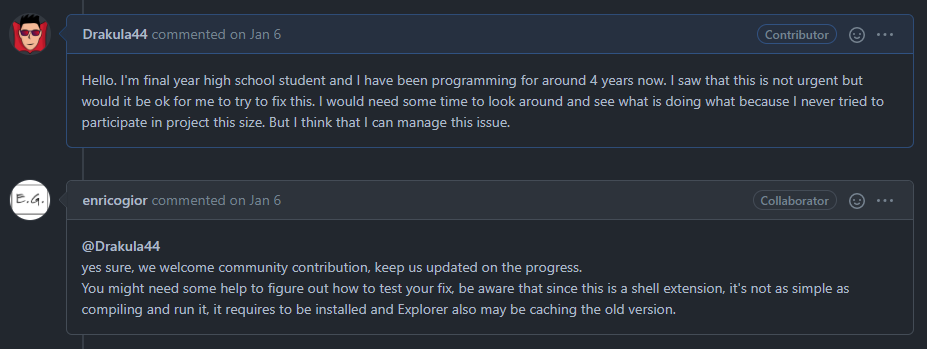
\includegraphics[scale=0.6]{prijava.png}
    \caption{Komunikacija sa administratorima repozitorijuma}
    \label{fig:prijava}
\end{figure}

\section{Identifikacija i reshavanje problema}
Kako bi kasnije mogli da napravimo {\latin pull request}, to jest da zatrazhimo da se nasha nadogradnja programa spoji sa glavnom verzijom moramo da napravimo {\latin fork} projekta na {\latin Github}-u. Taj {\latin fork} je potrebno preuzeti lokalno. U git-u komnda {\latin git clone url} skida projekat sa zadate adrese i automat\-ski podasheva tu adresu kao udaljeni repozitorijum sa nazivom {\latin origin}.\par
{\latin SVG} fajlovi su tekstualni fajlovi koji mogu da se jave zasebno ili u sklopu {\latin HTML} fajlova. 
Testiranjem se dobija da c1e internet pretrazhivachi prikazati fajl isto kao i u prijavljenom problemu ali u sluchaju pretrazhivacha to je zheljeni nachin. Jedno od reshenja problema je dodavanje ili ukoliko vec1 postoji izmena atributa {\latin style} u kome mogu da se definishu kako c1e dati objekat biti renderovan. Skaliranje objekta u {\latin HTML} moguc1e je postavljanjem {\latin CSS} atributa {\latin max-width} i {\latin max-height} koji c1e dozvoliti da visina i shirina objekta bude maksimalno specifikovane shirine.
Centriranje se postizhe pomoc1u atributa:

{\latin
\begin{center}
\begin{lstlisting}[caption=centriranje elementa]
position: absolute; 
top: 50%; 
left: 50%; 
transform: translate(-50%, -50%);
\end{lstlisting}
\end{center}
}
Gde c1e se prvo gornja leva ivica postaviti na sredinu ekrana i onda c1e se atributom {\latin transform}  objekat translirati za pola njegove shirine levo i pola visine gore.
Ovo reshenje je validno ali biblioteka koja se koristi ne podrzhava dovoljno veliku verziju {\latin CSS} standarda u kome su se ovi atributi pojavili. Biblioteka je zasnovana na {\latin Internet Exporeru 8}. Atributi za {\latin IE8} koji pravilno skaliraju objekat su sledec1i:
{\latin
\begin{center}
\begin{lstlisting}[caption=skaliranje elementra]
 _height:expression(this.scrollHeight > {heightR} ? \" {height}\" : \"auto\");
 _width:expression(this.scrollWidth > {widthR} ? \"{width}\" : \"auto\");
\end{lstlisting}
\end{center}
}

gde su {\latin width} i {\latin height} vec1 nalaze medju atributima polaznog {\latin SVG} fajla.
Nakon komitovanja i slanja verzije na lichni {\latin fork} zatrazhuje se {\latin pull request} slika (\ref{fig:pr}).
\begin{figure}[H]
    \centering
    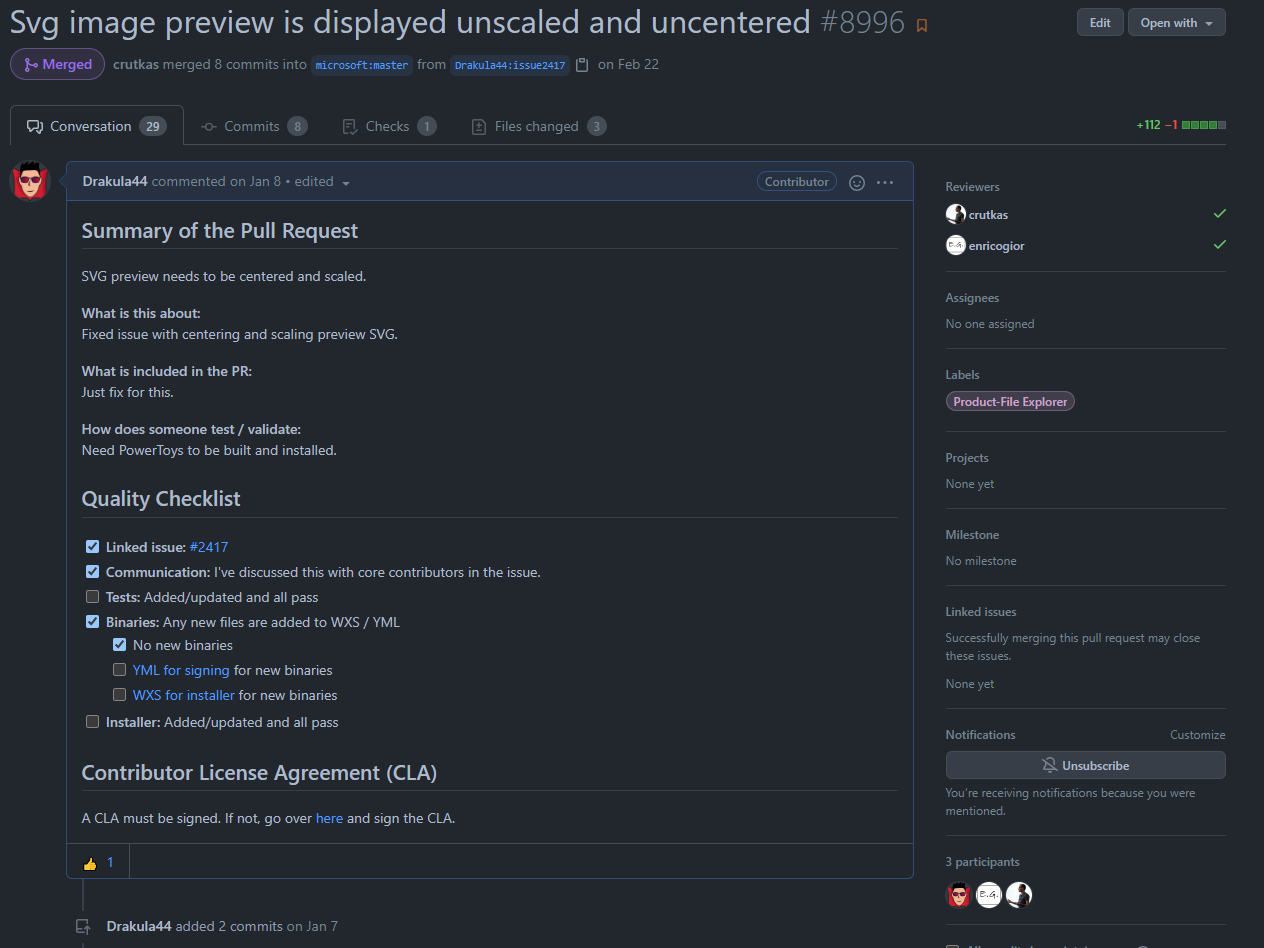
\includegraphics[scale=0.4]{pr1.png}
    \caption{Izgled napravljenog {\latin pull request}-a}
    \label{fig:pr}
\end{figure}
Nakon par interacija nad kodom. Uklanjanja napomenute greshke u vezi sa odgovarajuc1om verzijom {\latin CSS}-a, administratori repozitorijuma su spojili moju granu sa njihovom glavnom granom.
\begin{figure}[H]
    \centering
    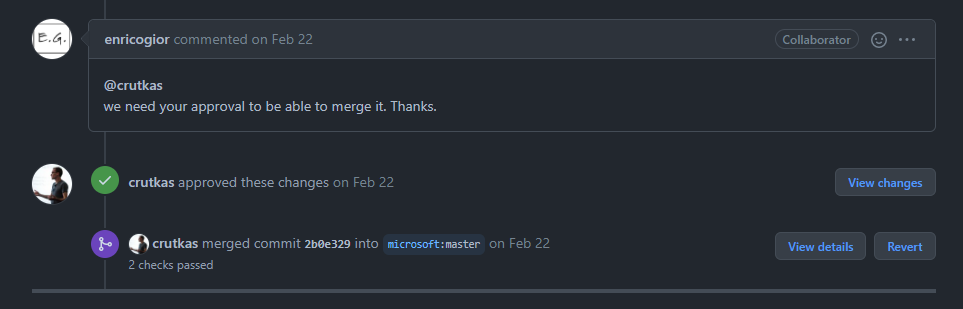
\includegraphics[scale=0.4]{pr2.png}
    \caption{Uspeshno spojeni {\latin pull request}}
    \label{fig:pr-approve}
\end{figure}

U sledec1oj verziji {\latin PoweraToys}-a u izveshtaju od arzhuriranju je bio i {\latin pull requst} koji sam ja odradio. Sa izashlom novom verzijom se zatvara i originalni problem.
\begin{figure}[H]
    \centering
    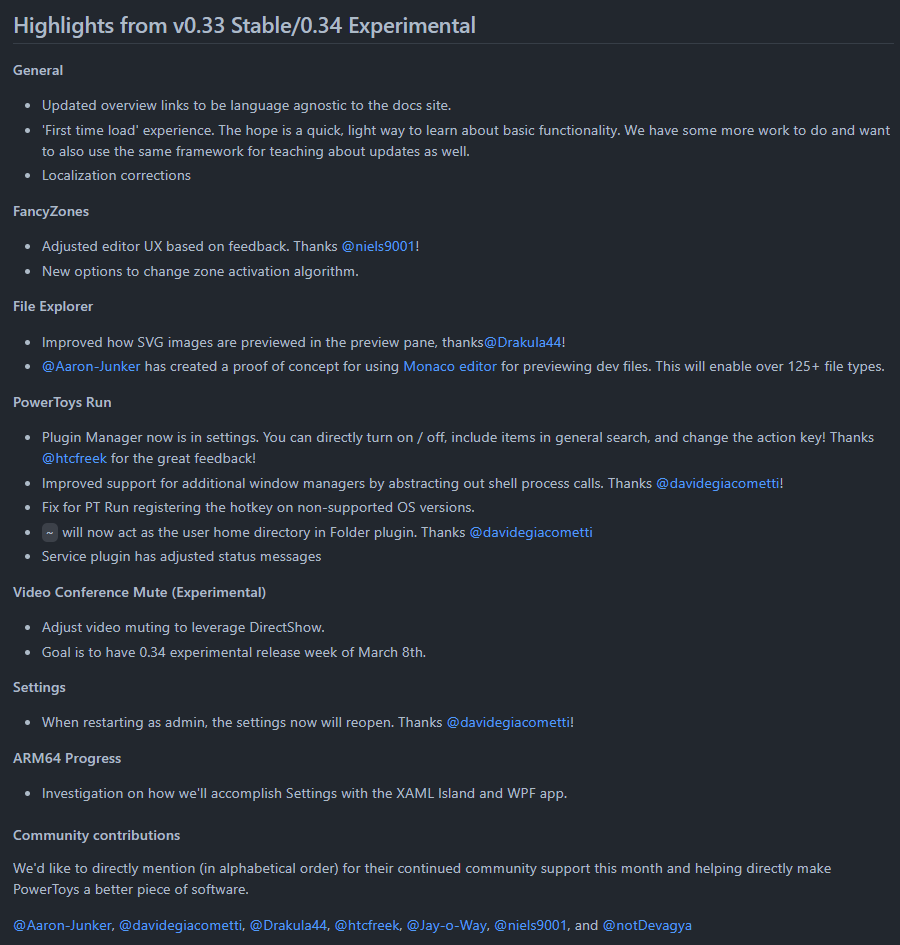
\includegraphics[scale=0.5]{izvestaj.png}
    \caption{Izveshtaj o promeni iz verzija kada se prvi put pojavljuje uradjena ispravka problema}
    \label{fig:izvestaj}
\end{figure}

\chapter[Shkolsko zvono]{Shkolsko zvono}
Kao poslednju demonstraciju pokazac1emo kako bi trebao da izgleda jedan kompletan projekat otvorenog koda. 
Pri kreiranju repozitorijuma na {\latin GitHub}-u (\ref{fig:pravljenje-rep}) moguc1e je dodati licencu. 
Za ovaj projekat izabrana je {\latin MIT License}. 
Ona omoguc1ava da bilo ko mozhe bez restrikcija koristiti kod u celini ili u njegovim delovima. 
Takodje daje obaveshtenje da za ovaj kod ne postoji garancija i da ga svako koristi na svoju odgovornost.\\

\fbox{
{\latin
\begin{minipage}{33em}
Permission is hereby granted, free of charge, to any person obtaining a copy
of this software and associated documentation files (the "Software"), to deal
in the Software without restriction, including without limitation the rights
to use, copy, modify, merge, publish, distribute, sublicense, and/or sell
copies of the Software, and to permit persons to whom the Software is
furnished to do so, subject to the following conditions:

The above copyright notice and this permission notice shall be included in all
copies or substantial portions of the Software.

THE SOFTWARE IS PROVIDED "AS IS", WITHOUT WARRANTY OF ANY KIND, EXPRESS OR
IMPLIED, INCLUDING BUT NOT LIMITED TO THE WARRANTIES OF MERCHANTABILITY,
FITNESS FOR A PARTICULAR PURPOSE AND NONINFRINGEMENT. IN NO EVENT SHALL THE
AUTHORS OR COPYRIGHT HOLDERS BE LIABLE FOR ANY CLAIM, DAMAGES OR OTHER
LIABILITY, WHETHER IN AN ACTION OF CONTRACT, TORT OR OTHERWISE, ARISING FROM,
OUT OF OR IN CONNECTION WITH THE SOFTWARE OR THE USE OR OTHER DEALINGS IN THE
SOFTWARE.
\end{minipage}
}}
\\\\
\par
\section{ Hardverskog reshenje}
Projekat je pokrenut na {\latin Raspberry Pi 3} modelu {\latin B}. 
Na njemu je moguc1e pokrenuti bilo koju modernu {\latin linux} distribuciju za {\latin ARM} arhitekturu. 
{\latin Raspberry Pi 3} u sebi sadrzi periferije niskog nivoa pomc1u kojih je moguc1e softverski pustiti ili prekinuti dotok struje. Napon struje mozhe da bude {\latin $0V$} ili {\latin $5V$}. Periferije niskog nivoa se nazivaju {\latin GPIO} pinovi. Kako bi smo kontrolisali zvono koje je povezano na mrezhu od {\latin $220V$} koristimo relej. Relej je elektrichna komponenta koja mozhe da zatvori ili otvori elektrichno kolo pomoc1u elektro magneta. Dovodjenem napona od $5v$ do elektro magneta relej c1e zatvoriti kolo i pokrenuti zvono. Kako bi se bezbedno pristupalo aplikaciji za konfiguraciju zvona napravljena je lokalna mrezha na koju je povezan {\latin Raspberry Pi} i osoba koja treba da podesi zvono slika (\ref{fig:shema_kola}).
\begin{figure}
    \centering
    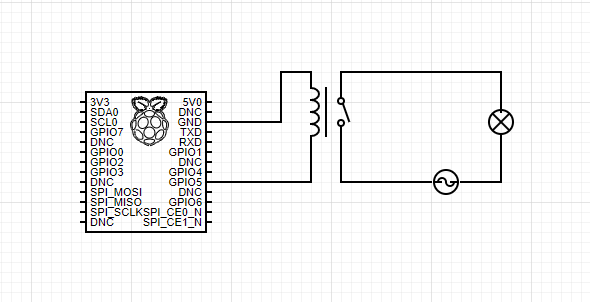
\includegraphics{shema.png}
    \caption{Elektronska shema shkolskog zvona}
    \label{fig:shema_kola}
\end{figure}

\section{Softversko reshenje}

Projekat se mozhe podeliti na tri dela:
\begin{itemize}
    \item Internet stranica za kontrolu zvona
    \item Pamc1enje i izvrshavanja zadataka - zvonjenje
    \item Kontrola {\latin GPIO} pinova
\end{itemize}

\subsection{Stranica za kontrolu zvona}
Kontrola zvona se vrshi sa stranice koja je hostovana pomoc1u {\latin Flask} modula. Kako bismo pokrenuli {\latin Flask} aplikaciju potrebno je da u komandnoj liniji podesimo variablu:
{\latin
\begin{center}
\begin{lstlisting}[caption=Podeshavanje promenjivih]
export FLASK_APP=main.py
\end{lstlisting}
\end{center}
}
gde je {\latin main.py} fajl u kome se nalazi aplikacija.
Pokretanje aplikacije izvrshava se sledec1om komandom:
{\latin
\begin{center}
\begin{lstlisting}[caption={\latin flask run}]
flask run --host=0.0.0.0
\end{lstlisting}
\end{center}
}
Gde parametar {\latin host} oznachava da zhelimo da prihvatimo zahteve sa svih {\latin IP} adresa. Aplikacija c1e podrazumevno da slusha na portu 5000.\par

Folder u kome se nalazi {\latin Flask} aplikacija mora da poseduje odredjene foldere:
\begin{itemize}
    \item {\latin static} u njemu se chuvaju svi {\latin CSS} i {\latin Javascript} fajlovi
    \item {\latin templates} u njemu su shabloni {\latin HTML} fajlova pisani u {\latin Jinja2} formatu.
\end{itemize}

Inicijalizacija {\latin Flask} projekata:
{\latin
\begin{center}
\begin{lstlisting}[language=Python,caption=inicijalizacija aplikacije]
from flask import Flask
from flask import render_template,request,url_for,redirect
from flask_assets import Environment

app = Flask(__name__)
assets = Environment(app)
assets.register(data.bundles)
\end{lstlisting}
\end{center}
}

Prvo napravimo glavni meni koji je na linku / to jest u korenu samog sajta. 
Glavni meni sadrzhi dva linka. 
Jedan je ka strani gde mozhemo da promeni trenutni nedeljni raspored chasova.
Drugi pomoc1u koga palimo ili gasimo sistem za kontrolu zvona.

{\latin
\begin{center}
\begin{lstlisting}[language=Python,caption=Pochetna strana]
@app.route('/')
def index():
    return render_template('index.html',working=data.working)
\end{lstlisting}
\end{center}
}

gde je {\latin index.html} shablon po kome se sajt pravi a {\latin working} promenjiva da li trenutno radi zvono.

{\latin
\begin{center}
\begin{lstlisting}[language=HTML,caption={\latin index.html}]
<!doctype html>
<title>Zvono</title>
<ul >
    <li>
        <a href="/raspored" style="font-size: 40px;">Promenite raspored</a>
    </li>
    
    <a href="/toggle" style="font-size: 40px;">Ugasite zvono</a>
    
    
    <a href="/toggle" style="font-size: 40px;">Uplatite zvono</a>
    
</ul>
</body>
</html>
\end{lstlisting}
\end{center}
}
Primetimo da {\latin Jinja2} format dodaje logiku koja je po sintaksi slicha {\latin Python} programskom jeziku. Pomoc1u nje proveravamo da li sistem za upravljanje zvonom radi i ispisujemo pravilnu poruku.

Strana za kontrolu zvona nalazi se na linku {\latin /raspored}. Rasporedu prosljedjujemo trenutni nedeljni raspored kao i imena dana u nedelji.
{\latin
\begin{center}
\begin{lstlisting}[language=Python]
@app.route('/raspored')
def weekly_schedule():
    return render_template('raspored.html',raspored=data.weekly_schedule,diw=data.days_in_week)
\end{lstlisting}
\end{center}
}

{\latin
\begin{center}
\begin{lstlisting}[language=HTMLcaption={\latin raspored.html}]
<body>
<form action="/submit" method="post" style="display: flex; flex-direction: column;">
    <ul id="nav_section">
        
            <li id="timeEntry-{{ i }}">
            <ul>
            
                    <h3>{{ diw[i] }}</h3>
            
            </ul>
            
            <ul id="timeEntry-{{ i }}_{{ j }}">
                    <input onclick="removeRow(this)" type="button" value="X" id="timeEntry-{{ i }}_{{ j }}" class="removeButton"><br>
                    Od:<input type="time" id="timeEntryfirst-{{ i }}_{{ j }}" name="timeEntryfirst-{{ i }}_{{ j }}"
                    value="{{ raspored[i][j][0] }}"><br>
                Do:<input type="time" id="timeEntrysecond-{{ i }}_{{ j }}" name="timeEntrysecond-{{ i }}_{{ j }}"
                    value="{{ raspored[i][j][1] }}">
                </ul>
                
            <ul id="button-{{ i }}">
            <input onclick="addRow(this)" type="button" value="Dodajte novi cas" id="addNew-{{ i }}">
            </ul>
            </li>
        
    </ul>
    <input type="submit" value="Promenite raspored" class="submit" style="font-size: 50px;">
</form>
</body>
\end{lstlisting}
\end{center}
}
Glavni deo strane raspored predstavlja forma koju generishemo pomoc1u postojec1eg rasporeda. Promenjiva {\latin raspored} je lista od 7 listi gde je svaka lista proizvoljne duzhine. Elementi liste su parovi dva vremenena - pochetak i zavrshetak chasa. U svakoj koloni postoji dugme \textit{Dodajte novi chas} koji pokrec1e funkciju u {\latin JavaScript}-u {\latin addRow(el)}

{\latin
\begin{center}
\begin{lstlisting}[caption={\latin addRow(element)}]
function addRow(element) {
  var beforeId = document.getElementById(element.id).parentElement.previousElementSibling.id;
  var newId;
  if(beforeId)
  {
    newId = beforeId.split("_")[0].concat("_");
    newId = newId.concat((parseInt(beforeId.split("_")[1])+1).toString());
  }
  else
  {
    newId = document.getElementById(element.id).parentElement.parentElement.id.concat("_0");
  }
  var firstid = newId.split("-")[0] + "first-" +newId.split("-")[1]
  var secondid = newId.split("-")[0] + "second-" +newId.split("-")[1]
  var newEntry = $( `<ul id="${newId}"><input onclick="removeRow(this)" type="button" value="X" id="${newId}" class="removeButton"><br>Od:<input type="time" id="${firstid}" name="${firstid}"><br>Do:<input type="time" id="${secondid}" name="${secondid}"></ul>`);
  newEntry.insertBefore("#".concat(document.getElementById(element.id).parentElement.id))
  }
\end{lstlisting}
\end{center}
}

Funkcija {\latin addRow(element)} gleda predhodni element i generishe id za novi element koji c1e biti u formatu {\latin timeEntry-i\_j } gde su {\latin i} i {\latin j} pozicije elementa u listi. Moguc1e je izbrisati chas pomoc1u funkcije {\latin removeRow(ele)} koja se pokrec1e pritiskom na dugme pored.

{\latin
\begin{center}
\begin{lstlisting}[caption={\latin removeRow(element)}]
function removeRow(element)
{
  parentId =  document.getElementById(element.id);
  console.log(parentId.parentElement)
  $("#".concat(parentId.id)).remove();
}
\end{lstlisting}
\end{center}
}
Funkcija c1e izbrisati roditeljski element dugmeta to jest jedan chas.

\subsection{Izvrshavanje i kontrola zvonjenja}
Za planiranje izvrshavanja radnji koristimo modul {\latin schedule}.
Kako bi modul mogao da radi ne meshajuc1i se sa poslovima sajta potrebno je da ga pokrenemo u drugom tredu.

{\latin
\begin{center}
\begin{lstlisting}[language=Python]
def run_continuously(interval=1):
    cease_continuous_run = threading.Event()

    class ScheduleThread(threading.Thread):
        @classmethod
        def run(cls):
            while not cease_continuous_run.is_set():
                schedule.run_pending()
                time.sleep(interval)

    continuous_thread = ScheduleThread()
    continuous_thread.start()
    return cease_continuous_run

stop_run_continuously = run_continuously()
\end{lstlisting}
\end{center}
}

Prilikom prihvac1anja forme sa {\latin /raspored} dobijamo {\latin python} rechink u kome je svako vreme vezano za id polja iz kojeg je. Pomoc1u funkcije {\latin dict\_to\_array} konvertujemo taj rechink u listu listi koju ostatk programa trazhi.

{\latin
\begin{center}
\begin{lstlisting}[language=Python]
def dict_to_array(dict):
    niz = data.weekly_schedule
    for i in range(7):
        niz[i] = []
        j = 0
        key_first = "timeEntryfirst-" + str(i) + "_" + str(j)
        key_second = "timeEntrysecond-" + str(i) + "_" + str(j)
        while key_first in dict and key_second in dict:
            if dict[key_first] != '' and dict[key_second] != '':
                niz[i].append([dict[key_first],dict[key_second]])
            j+=1
            key_first = "timeEntryfirst-" + str(i) + "_" + str(j)
            key_second = "timeEntrysecond-" + str(i) + "_" + str(j)
        data.weekly_schedule = niz
        refresh_schedule()
\end{lstlisting}
\end{center}
}

Na kraju funkcije pokrec1emo funkciju {\latin refresh\_schedule} koja c1e za svako vreme i odgovarajuc1i dan pokrenuti funkciju gde je dan iz skupa {\latin (monday, tuesday, wednesday, thursday, friday, saturday, sunday)}.

{\latin
\begin{center}
\begin{lstlisting}[language=Python,caption=planiranje izvrshavanja funkcije]
schedule.every().dan.at(vreme[broj_dana][j][k]).do(ring_bell)
\end{lstlisting}
\end{center}
}

\subsection{Kontrola {\latin GPIO} pinova}
Na pochetku programa inicijalizujemo pin 17 to jest {\latin GPIO} pin 6.

{\latin
\begin{center}
\begin{lstlisting}[language=Python]
import RPi.GPIO as GPIO
GPIO.setmode(GPIO.BCM)
GPIO.setup(17, GPIO.OUT)
\end{lstlisting}
\end{center}
}

Funkciom {\latin ring\_bell} postavljamo {\latin GPIO} pin 6  na $5V$ u trajanju od 3,5 sekundi i nakon toga ga vrac1amo na $0V$.

{\latin
\begin{center}
\begin{lstlisting}[language=Python]
def ring_bell():
    GPIO.output(17, GPIO.HIGH)
    time.sleep(3.5)
    GPIO.output(17, GPIO.LOW)
\end{lstlisting}
\end{center}
}

\chapter{Zakljuchak}
Cilj rada je bio:
\begin{itemize}
    \item da se pokazhe razvoj programiranja otvorenog koda kroz vreme i ukazhe na njegove prednosti.
    \item pregled tehnologije koje su potrebne da bi programiranje otvorenog koda bilo efikasno.
    \item Pomaganje projektu {\latin PowerToys} koje je pomoglo korsnicima aplikacije.
    \item Izrada sistema za shkolsko zvono koje u vreme pisanja radi u Matematichkoj gimnaziji.
\end{itemize}
Uz prednosti programiranje otvorenog koda, ovaj pristup ima potencijal da prevlada u odnosu na zatvoreni kod ali ne mozhe skroz da ga zameni. \par {\latin PowerToys} program se nalazi na {\latin Github}\footnote{{\latin https://github.com/microsoft/PowerToys}}-u.\par
Sistem za shkolsko zvono mozhe se nac1i na {\latin Github}\footnote{{\latin https://github.com/Drakula44/skolsko\_zvono}}-u kao i kompletna dokumentacija za kod i korisnichko upustvo. Svaka pomoc1 pri unapredjenju projekta je dobrodoshla.
\\\par 
Hteo bih da se zahvalim :
\begin{itemize}
    \item svom mentoru Mijodragu Djurishic1u za pomoc1 pri pisanju maturskog rada
    \item {\latin Enrico Giordani} i {\latin Clint Rutkas} pri pomoc1i pri realizaciji {\latin pull requst}-a za {\latin PowerToys}
\end{itemize}


%\renewcommand*{\biblname}{}
\renewcommand\bibname{ Literatura}
 \addcontentsline{toc}{chapter}{ Literatura}



\begin{thebibliography}{7}
\vspace*{15mm}
\rm

\bibitem{M} {\latin Raymond, Eric. "The cathedral and the bazaar." Knowledge, Technology \& Policy 12.3 (1999): 23-49.}
% https://github.com/microsoft/PowerToys/pull/8996
% 
\bibitem{M} {\latin https://opensource.org/}
\bibitem{M} {\latin https://flask.palletsprojects.com/en/2.0.x/quickstart/}
\bibitem{M} {\latin https://jinja.palletsprojects.com/en/3.0.x/}
\bibitem{M} {\latin https://pypi.org/project/schedule/}


\end{thebibliography}

\ape
\chapter{Dodatak}
\section*{Pregled promena koje su napravljene u {\latin pull request}-u za projekat {\latin PowerToys}}

{\latin
\begin{center}
    \begin{lstlisting}[language=csh,caption={\latin src/modules/previewpane/SvgPreviewHandler/Utilities/SvgPreviewHandlerHelper.cs }]

        /// <summary>
        /// Add proper
        /// </summary>
        /// <param name="stringSvgData">Input Svg</param>
        /// <returns>Returns modified svgData with added style</returns>
        public static string AddStyleSVG(string stringSvgData)
        {
            XElement svgData = XElement.Parse(stringSvgData);

            var attributes = svgData.Attributes();
            string width = string.Empty;
            string height = string.Empty;
            string widthR = string.Empty;
            string heightR = string.Empty;
            string oldStyle = string.Empty;

            // Get width and height of element and remove it afterwards because it will be added inside style attribute
            for (int i = 0; i < attributes.Count(); i++)
            {
                if (attributes.ElementAt(i).Name == "height")
                {
                    height = attributes.ElementAt(i).Value;
                    attributes.ElementAt(i).Remove();
                    i--;
                }
                else if (attributes.ElementAt(i).Name == "width")
                {
                    width = attributes.ElementAt(i).Value;
                    attributes.ElementAt(i).Remove();
                    i--;
                }
                else if (attributes.ElementAt(i).Name == "style")
                {
                    oldStyle = attributes.ElementAt(i).Value;
                    attributes.ElementAt(i).Remove();
                    i--;
                }
            }

            svgData.ReplaceAttributes(attributes);

            height = CheckUnit(height);
            width = CheckUnit(width);
            heightR = RemoveUnit(height);
            widthR = RemoveUnit(width);

            string centering = "position: absolute; top: 50%; left: 50%; transform: translate(-50%, -50%);";

            // Because WebBrowser class is based on IE version that do not support max-width and max-height extra CSS is needed for it to work.
            string scaling = $"max-width: {width} ; max-height: {height} ;";
            scaling += $"  _height:expression(this.scrollHeight > {heightR} ? \" {height}\" : \"auto\"); _width:expression(this.scrollWidth > {widthR} ? \"{width}\" : \"auto\");";

            svgData.Add(new XAttribute("style", scaling + centering + oldStyle));
            return svgData.ToString();
        }

        /// <summary>
        /// If there is a CSS unit at the end return the same string, else return the string with a px unit at the end
        /// </summary>
        /// <param name="length">CSS length</param>
        /// <returns>Returns modified length</returns>
        private static string CheckUnit(string length)
        {
            string[] cssUnits = { "cm", "mm", "in", "px", "pt", "pc", "em", "ex", "ch", "rem", "vw", "vh", "vmin", "vmax", "%" };
            foreach (var unit in cssUnits)
            {
                if (length.EndsWith(unit, System.StringComparison.CurrentCultureIgnoreCase))
                {
                    return length;
                }
            }

            return length + "px";
        }

        /// <summary>
        /// Remove a CSS unit from the end of the string
        /// </summary>
        /// <param name="length">CSS length</param>
        /// <returns>Returns modified length</returns>
        private static string RemoveUnit(string length)
        {
            string[] cssUnits = { "cm", "mm", "in", "px", "pt", "pc", "em", "ex", "ch", "rem", "vw", "vh", "vmin", "vmax", "%" };
            foreach (var unit in cssUnits)
            {
                if (length.EndsWith(unit, System.StringComparison.CurrentCultureIgnoreCase))
                {
                    length = length.Remove(length.Length - unit.Length);
                    return length;
                }
            }

            return length;
        }
    \end{lstlisting}
\end{center}
}
\clearpage
{\latin
\begin{center}
    \begin{lstlisting}[caption={\latin src/modules/previewpane/SvgPreviewHandler/SvgPreviewControl.cs }]
            try
            {
                svgData = SvgPreviewHandlerHelper.AddStyleSVG(svgData);
            }
#pragma warning disable CA1031 // Do not catch general exception types
            catch (Exception ex)
#pragma warning restore CA1031 // Do not catch general exception types
            {
                _browser.ScrollBarsEnabled = true;
                PowerToysTelemetry.Log.WriteEvent(new SvgFilePreviewError { Message = ex.Message });
            }
...
            _browser.ScrollBarsEnabled = false;
    \end{lstlisting}
\end{center}
}

\end{document}
